%%\documentclass[aspectratio=1610]{beamer}
\documentclass[xcolor=table,xcolor=dvipsnames]{beamer}
%
%%%%%%%%%%%%%%%%%%%%%%%%%%%%%%%%%%%%
%% Common preamble
%%%%%%%%%%%%%%%%%%%%%%%%%%%%%%%%%%%%
% PAGE
%% \usepackage{fullpage}
% FONTS
\usepackage{booktabs} % provides toprule, bottomrule, midrule
\usepackage{lmodern} % enhanced version of computer modern
\usepackage[T1]{fontenc} % for hyphenated characters
\usepackage{amssymb}
\usepackage{mathtools} % contains amsmath which comes with align
\usepackage{amsthm}
\usepackage{microtype} % some compression
%%%%%%%%%%%%%%%%%%%%%%%%%%%%%%%%%%%%
\usepackage{tikz}
\usepackage{multirow}
\usetikzlibrary{spy,shadows,arrows,shapes,positioning,calc,backgrounds,fit,automata}
\newcommand{\lantanafull}{\emph{Lantana camara}}
\newcommand{\lantana}{\emph{L.~camara}}
\newcommand{\partheniumfull}{\emph{Parthenium hysterophorus}}
\newcommand{\parthenium}{\emph{P.~hysterophorus}}
\newcommand{\chromolaenafull}{\emph{Chromolaena odorata}}
\newcommand{\chromolaena}{\emph{C.~odorata}}


\newcommand{\completed}{\tikz{\draw[fill=green,opacity=1,line width=1pt] circle(1ex);}}
\newcommand{\ongoing}{\tikz{\draw[fill=yellow,opacity=1,line width=1pt] circle(1ex);}}
\newcommand{\notstarted}{\tikz{\draw[fill=red,opacity=1,line width=1pt] circle(1ex);}}

\newcommand{\newcompleted}{\tikz{\draw[fill=green,opacity=1,line width=1pt]
(-.2,-.2) rectangle (.15,.15);}}
\newcommand{\newongoing}{\tikz{\draw[fill=yellow,opacity=1,line width=1pt]
(-.2,-.2) rectangle (.15,.15);}}
\newcommand{\newnotstarted}{\tikz{\draw[fill=red,opacity=1,line width=1pt]
(-.2,-.2) rectangle (.15,.15);}}

\newcommand{\rowcon}[2]{\cellcolor{#2}\parbox{2cm}{\small #1}}

\newcommand{\dunder}[1]{\underline{\underline{#1}}}
\newcommand{\calc}{\mathcal{C}}
\newcommand{\cali}{\mathcal{I}}
\newcommand{\calb}{\mathcal{B}}
\newcommand{\calo}{\mathcal{O}}
\newcommand{\cals}{\mathcal{S}}
\newcommand{\calp}{\mathcal{P}}
\newcommand{\domb}{\mathbb{B}}
\newcommand{\dmax}{d_{\max}}
\newcommand{\cost}{\text{cost}}
\newcommand{\comment}[1]{{\color{red}#1}}
\newcommand{\wmin}{w_{\min}}
\newcommand{\copt}{C_{\text{OPT}}}
\newcommand{\TikZ}{Ti\textit{k}Z\xspace}
\newcommand{\tuta}{\emph{T. absoluta}}
\newcommand{\prempt}{\textsc{PREMpT}}
\definecolor{col1}{HTML}{D53E4F}
\definecolor{col2}{HTML}{F46D43}
\definecolor{col3}{HTML}{FDAE61}
\definecolor{col4}{HTML}{FEE08B}
\definecolor{col5}{HTML}{E6F598}
\definecolor{col6}{HTML}{ABDDA4}
\definecolor{col7}{HTML}{66C2A5}
\definecolor{col8}{HTML}{3288BD}


%%
\title[]{Assessment of Invasive Alien Plant Species Distribution in the Chitwan Annapurna Landscape (CHAL) region ,Nepal with the Application of satellite Imagery}
\date[July 14, 2020]{Jul 14, 2020}
\author[A.~Adiga]{Abhijin Adiga and Madhav Marathe (PI)}
\institute[]{
    \mbox{}\hspace{.9cm}\raisebox{.6cm}{\includegraphics[width=4cm]{figs/uva_horiz_rgb.png}}\hspace{.9cm}\raisebox{.2cm}{
\includegraphics[width=2.5cm]{figs/bivt_logo.pdf}}\\
\raisebox{.55cm}{\includegraphics[width=3.4cm]{figs/IPM-Innovation-Lab-header-logo.png}}~\hspace{.2cm}\raisebox{.4cm}{\includegraphics[width=3.4cm]{figs/FtF.pdf}}~\hspace{.2cm}\raisebox{.4cm}{\includegraphics[width=3.1cm]{figs/usaid.pdf}}
}
%% ----------------------------------------------------------------------
%%
\usetheme{CambridgeUS}
\useoutertheme{nssac}

%% This ``scales'' the font. Don't extend too much beyond 128x96
%% Uncomment the next line for default sizes:
\geometry{paperwidth=140mm,paperheight=105mm}
\setbeamercolor{block title}{use=structure,fg=white,bg=black!75!white}
\setbeamercolor{block body}{use=structure,fg=black,bg=black!10!white}
\beamertemplatenavigationsymbolsempty

\begin{document}
%% ----------------------------------------------------------------------

\begin{frame}
\titlepage
\end{frame}
%%
%% ----------------------------------------------------------------------
%%
\begin{frame}
\frametitle{Main objectives}
\begin{itemize}
\item Understand the multipathway spatiotemporal spread of multiple invasive plants in the CHAL region.
\item Understand how multiple invasive species coexist and compete.
\item Informing domain experts and policy makers
\begin{itemize}
    \item Routes of introduction and spread
    \item On pathways of spread
    \item Monitor and mitigate
\end{itemize}
\end{itemize}
To this end:
\begin{enumerate}
    \item Develop a deep learning based framework to create species
    distribution maps.
    \item Apply this framework along with network (agent-based) models to
    study the spatio-temporal spread of the focus invasive species.
\end{enumerate}
Team: 1 postdoc (Institute funds) + two interns (summer/Capstone project) + two
research scientists

\alert{Preliminary results presented in a conference held by American
Society for Photogrammetry and Remote Sensing (ASPRS).}
\end{frame}
%%
%% ---------------------------------------------------------------------- 
%%
\begin{frame}
\frametitle{Survey data} 
\begin{columns}[c]
\column{.5\textwidth}
\begin{itemize}
\item Objective: Mapping the distribution of three species.
\item Three phases: Sep. to Dec. 2018, Mar. to May 2019 and Sep. to Dec. 2020.
\item Often, the recorded coordinates do not correspond to the exact location of the plants.
\item Variation in spatial coverage: patchy to abundant, requiring high-resolution imagery.
\item Comparatively small dataset for training deep learning algorithms.
\item Seasonal variations in appearance (phenology)
\end{itemize}
\column{.5\textwidth}
\newcommand{\rom}[1]{\uppercase\expandafter{\romannumeral #1\relax}}
\begin{table}[t]
\centering
\scriptsize
%% \rowcolors{2}{white}{gray!15} % For this to work, put \PassOptionsToPackage{table}{xcolor} before \documentclass
\begin{tabular}{p{.25\textwidth}>{\centering\arraybackslash}p{.1\textwidth}>{\centering\arraybackslash}p{.1\textwidth}>{\centering\arraybackslash}p{.1\textwidth}}
\hline
{\bf Species} & {\bf Phase} & {\bf Total} & {\bf Presence}\\
\hline
\hline
\multirow{3}{*}{\lantana} &
\rom{1} &
156 &
70 \\
&
\rom{2} &
147 &
106 \\
&
\rom{3} &
369 &
196 \\
\hline
\multirow{2}{*}{\parthenium} &
\rom{2} &
179 &
96 \\
&
\rom{3} &
96 &
89 \\
\hline
\multirow{2}{*}{\chromolaena} &
\rom{2} &
112 &
49 \\
&
\rom{3} &
345 &
199 \\
\hline
\end{tabular}
\end{table}

\vspace{-.2cm}
\centering
\includegraphics[width=\textwidth]{figs/density.png}
\end{columns}
\end{frame}
%%
%% ---------------------------------------------------------------------- 
%%
\begin{frame}
\frametitle{Main idea} 
{
\centering
\includegraphics[width=\textwidth]{figs/idea.png}
}
\end{frame}
%%
%% ---------------------------------------------------------------------- 
%%
\begin{frame}
\frametitle{Main idea} 
{
\centering
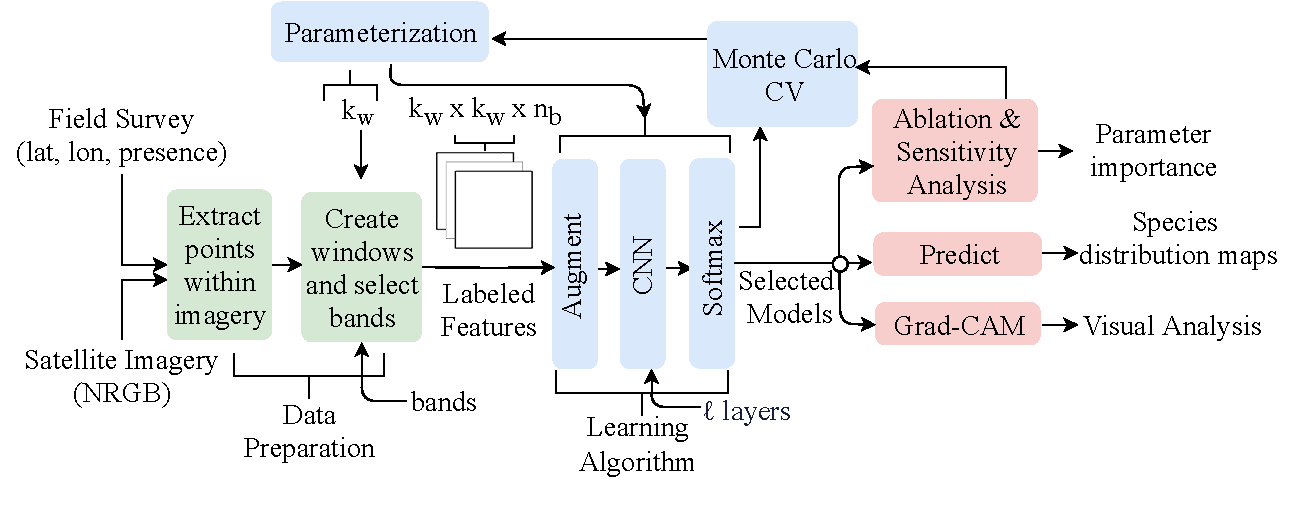
\includegraphics[width=\textwidth]{figs/full_architecture.pdf}
}
\end{frame}
%%
%% ---------------------------------------------------------------------- 
%%
\begin{frame}
\frametitle{Training and prediction performance}
\begin{columns}[c]
\column{.5\textwidth}
\begin{itemize}
\item Monte-Carlo cross validation: Multiple (train,validation,hold-out) sets.
\item Hyperparameter tuning: Gradient Boosted Regression Trees: learning rate, batchsize, architecture (depth and number of filter layers), dropout, maxpooling and augmentation.
\item Loss functions: binary cross-entropy, squared hinge
\item Compute nodes with 2 x Intel(R) Xeon(R) Gold 6248 CPU @ 2.50GHz processors with 20 cores per cpu; 386GB memory; and 4xNVIDIA Volta V100 GPUs.
\end{itemize}
\column{.5\textwidth}
\begin{tabular}{lrr}
\toprule
      Species &  $k_w$ &  F1 Score \\
\midrule
 \chromolaena &     32 &          0.736 \\
 \chromolaena &     64 &          0.755 \\
 \chromolaena &    128 &          0.785 \\
     \lantana &     16 &          0.731 \\
     \lantana &     32 &          0.768 \\
     \lantana &     64 &          0.798 \\
     \lantana &    128 &          0.804 \\
  \parthenium &     32 &          0.946 \\
  \parthenium &     64 &          0.960 \\
  \parthenium &    128 &          0.963 \\
\bottomrule
\end{tabular}

\end{columns}
\end{frame}
%%
%% ---------------------------------------------------------------------- 
%%
\begin{frame}
\frametitle{Explaining the classification: GradCam analysis} 
\begin{itemize}
    \item Gradient Weighted-Class Activation Map (Grad-CAM) [Selvaraju et al. 2017] is a very popular technique used to discover patterns in the image that were used by the deep learner to classify the image.
    \item TP: True positive; TN: True negative; HS: Human settlement; NHS: Not HS.
\end{itemize}
\centering
\includegraphics[width=.9\textwidth]{figs/gradcam.png}
\end{frame}
%%
%% ---------------------------------------------------------------------- 
%%
\end{document}
